\documentclass[11pt]{article}
\usepackage[T1]{fontenc}
\usepackage{lmodern}
\usepackage[a4paper, margin=2cm]{geometry}
\usepackage{graphicx}
\usepackage{amsmath}
\usepackage{xcolor}
\usepackage{booktabs}
\usepackage[hidelinks]{hyperref}
\title{TrueJES: the jet energy scale along the truth ladder\\[4pt]\large illustrations}
\author{Reco2Pico / analysis/TrueJES}
\date{\today}
\begin{document}
\maketitle

\section*{1. The ladder}
One jet collection per step, all built on the same simulated events and all
matched to the same generator jet. The difference of the response between two
consecutive steps isolates one effect; the last rung is the Puppi jet with the
GlobalTag corrections, i.e. what an analysis sees.
\begin{center}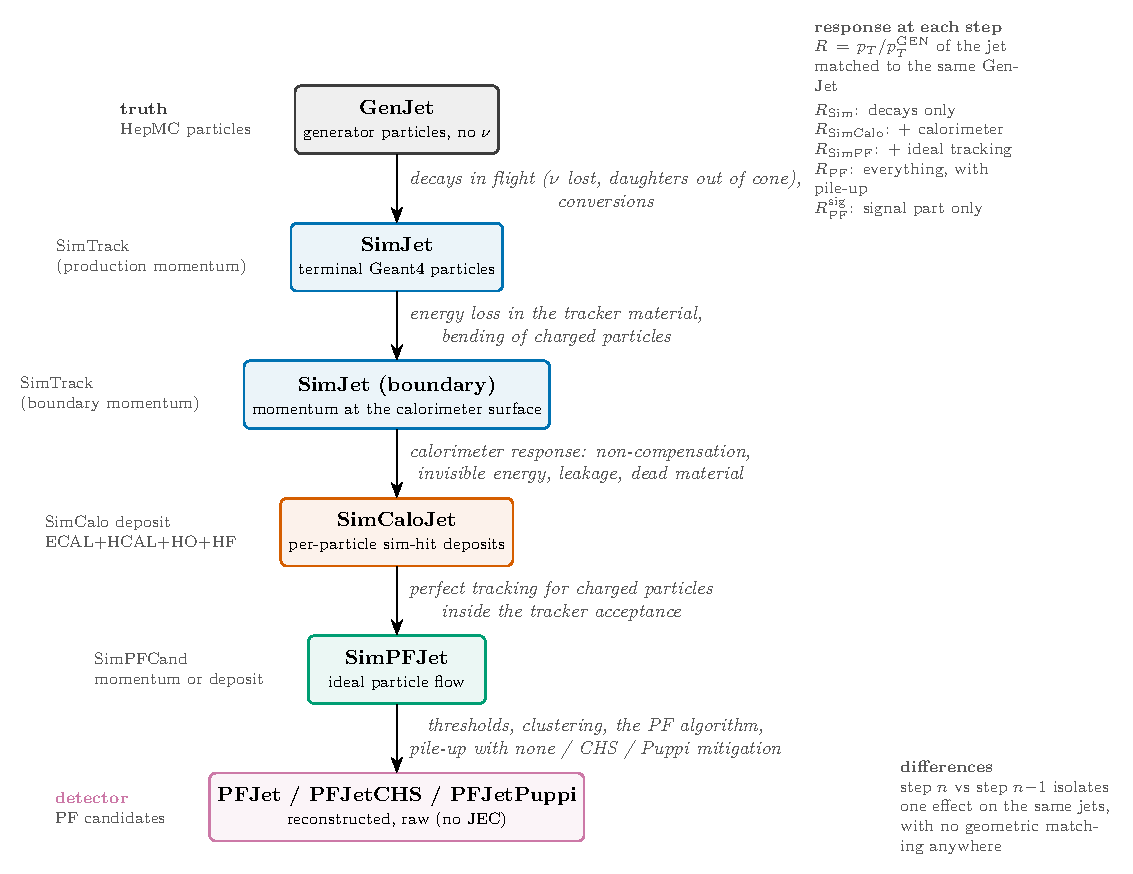
\includegraphics[width=\textwidth]{ladder.pdf}\end{center}

\section*{2. Matching by ancestry, not by $\Delta R$}
Every Geant4 particle descends from one generator primary, and every generator
particle sits in at most one gen jet. The energy a jet shares with a gen jet is
therefore exact, whatever the magnetic field and the decays did to the
directions. The same scores are used at every step.
\begin{center}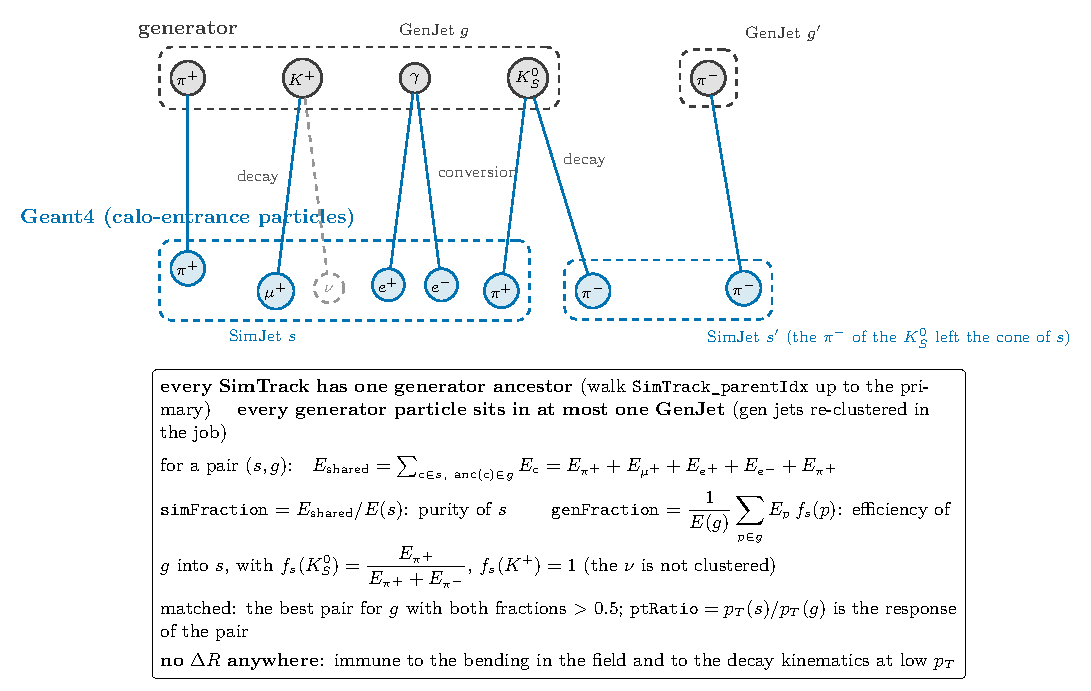
\includegraphics[width=\textwidth]{ancestry_matching.pdf}\end{center}

\section*{3. Which Geant4 particles are clustered}
The calorimeter-entrance particles: the cut through the stored decay tree at
the tracker/calorimeter boundary, after the decays, conversions, energy loss
and bending in the tracker. Geant4's crossing flag alone does not give it (a
stored secondary born in the tracker never carries it, and the sim hits of a
daughter born inside the calorimeter reference the daughter), so the flag, the
production vertex and the ownership of the sim hits are combined, and every
hit is bookkept to exactly one entrance particle. The same list defines the
sim jets (production momenta, and at the face), the deposits and the ideal
particle-flow list.
\begin{center}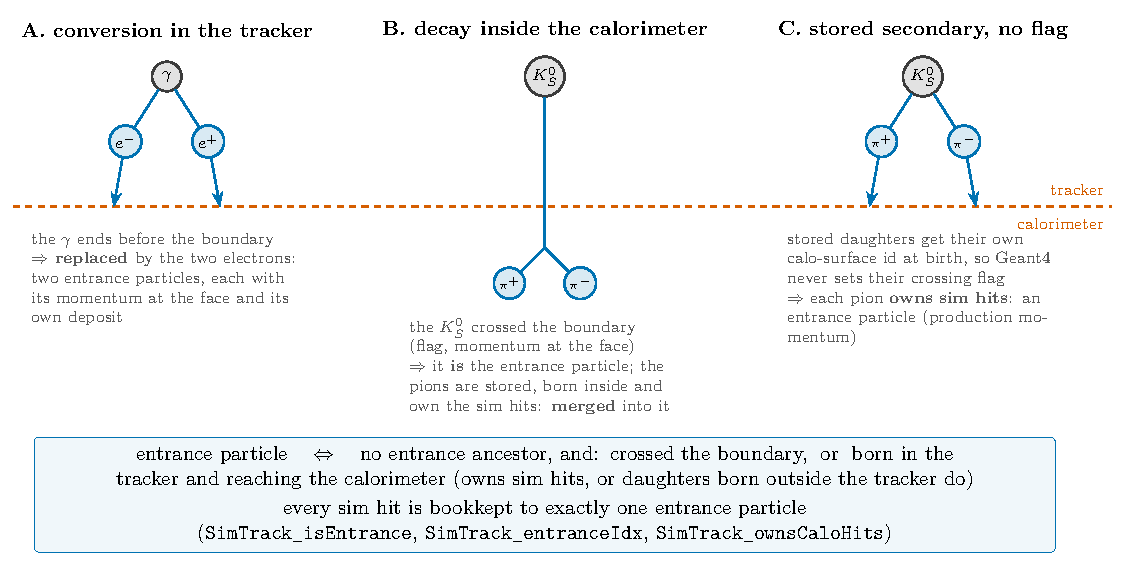
\includegraphics[width=\textwidth]{entrance_rule.pdf}\end{center}

\section*{4. The calorimeter response from the sim hits}
The calorimeter sim hits carry the Geant4 id on the calorimeter surface, which
is mapped to the entrance particle, so the deposits are summed per particle
without clustering; jets of the deposits give the calorimeter-only response,
jets of the cells the same energy with the calorimeter geometry, and an ideal
particle flow built from momenta and deposits shows what tracking recovers.
\begin{center}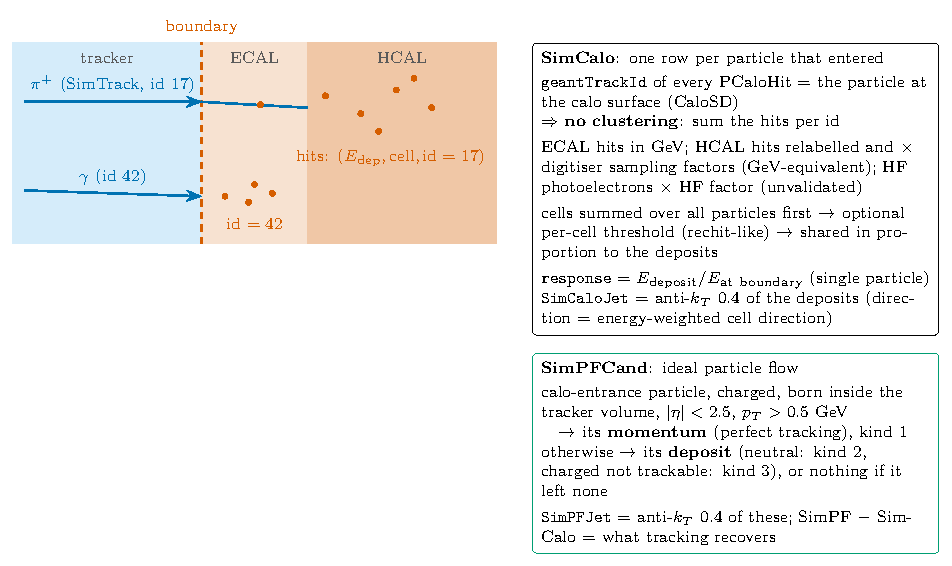
\includegraphics[width=\textwidth]{calo_deposits.pdf}\end{center}

\section*{5. The reconstructed jets on the same ladder}
PF candidates are attributed to simulated particles (track association for
charged ones, sim-hit shares of the cluster cells for the others); what is not
attributed is pile-up, noise or fakes. The reconstructed jets are then matched
by the same ancestry scores, and the signal-only response separates the
pile-up from the reconstruction effects without matching pile-up conditions.
\begin{center}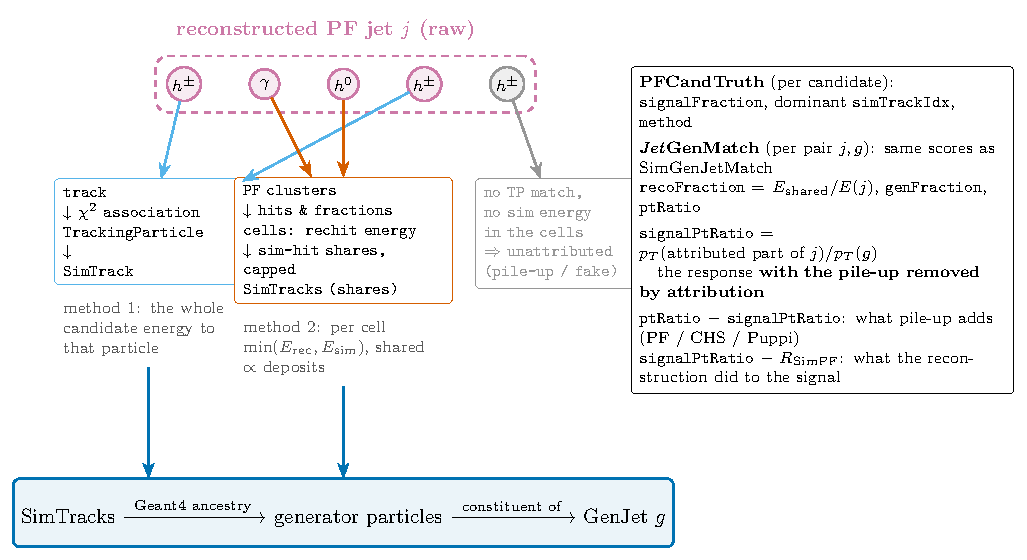
\includegraphics[width=\textwidth]{reco_attribution.pdf}\end{center}

\section*{6. From the jet down to the cell}
Everything the reconstruction side of the ladder uses is taken apart to the
rechits: the jet to its candidates (with their clustering weights), each
candidate to the block elements it was built from, a track for the charged
ones and the PF clusters otherwise, each cluster to its rechits with their
fractions. The rechit is one cell, and in that cell the Geant4 deposits are
known per calorimeter-entrance particle of the signal and per pile-up
particle. The attribution is made there, cell by cell, and summed back up the
same chain to the candidate and the jet; the track side goes through the
TrackingParticle instead. The rechit itself is the pulse fit of the digitised
samples, so noise, out-of-time pile-up and the calibration stay in the
residual.
\begin{center}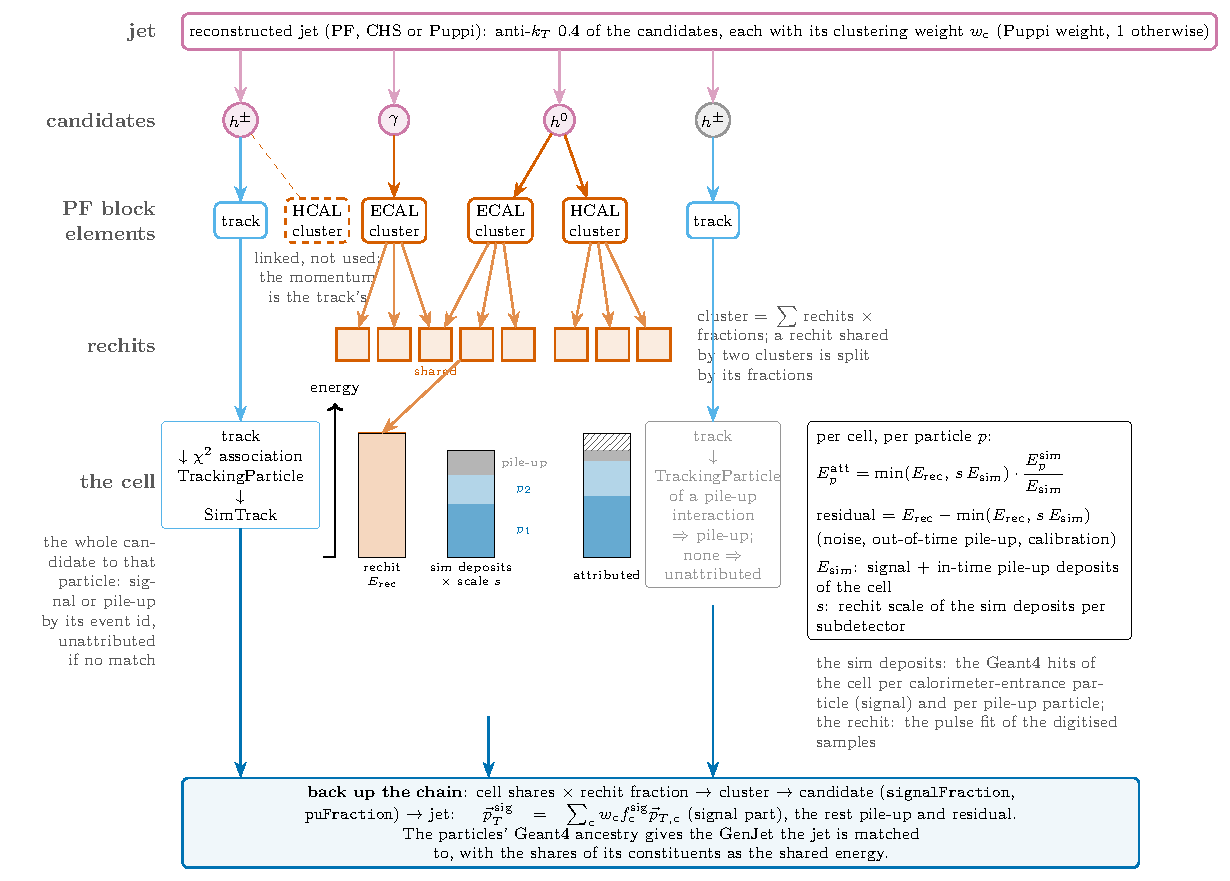
\includegraphics[width=\textwidth]{attribution_chain.pdf}\end{center}

\section*{7. How the pile-up is removed: attribution, not subtraction}
Every PF candidate is split into the part that can be traced to a simulated
particle of the hard-scatter event and a remainder. Charged candidates are
traced through their track, one object with one momentum. Neutral ones are
traced cell by cell: the cell is the finest unit the reconstruction and the
simulation share (the rechit is one number per cell, the sim hits say who
deposited how much in it), anything coarser needs a shower-shape assumption,
anything finer has no reconstructed counterpart. Within a cell the
reconstructed energy, capped by the simulated one on the rechit scale, is
shared in proportion to the deposits, which is the only unbiased statement
left once the fluctuation of a cell cannot be assigned to a particle. The
remainder is pile-up, noise or a fake. The signal part of a jet is the sum of
the traced parts of its constituents, so no pile-up matching between samples
is needed.
\begin{center}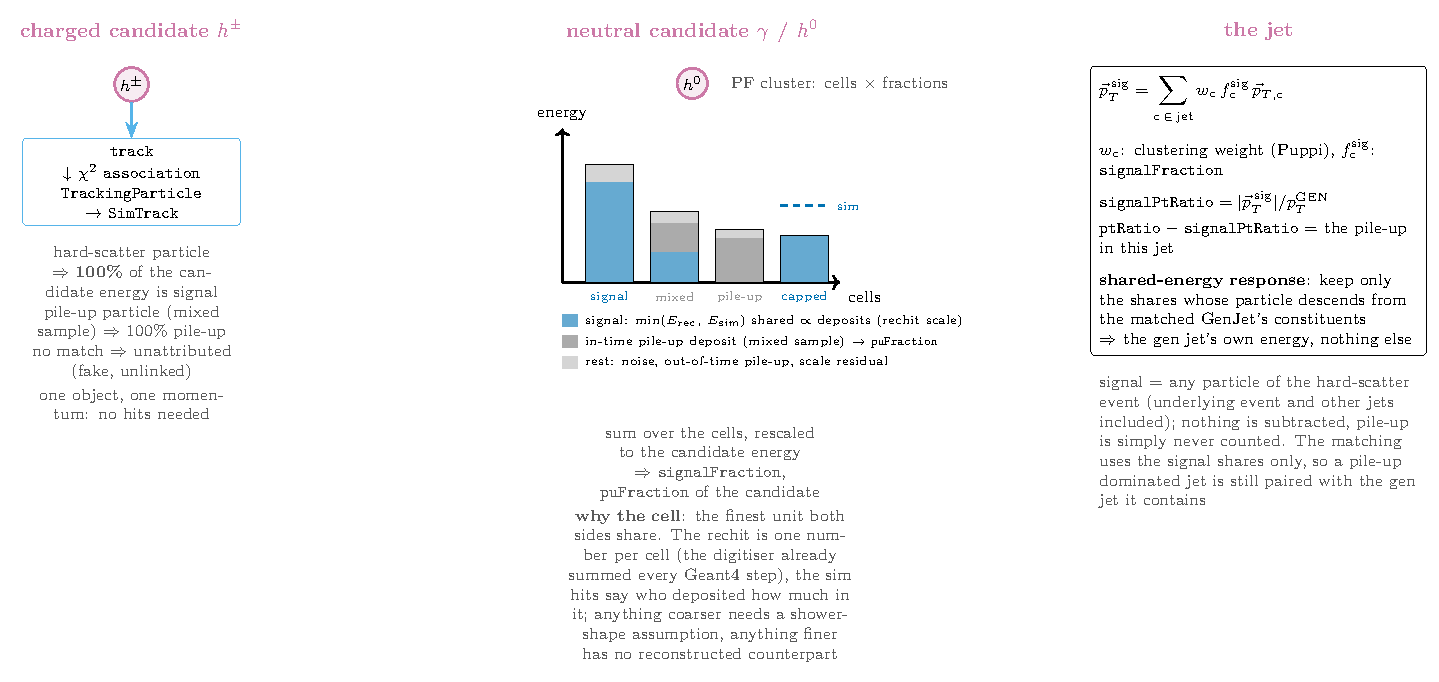
\includegraphics[width=\textwidth]{pileup_attribution.pdf}\end{center}

The same attribution runs on both kinds of sample. On the premixed one the
simulation knows the hard-scatter particles only, so the cap is the signal
deposit and everything unattributed is ``pile-up'' in one number: in-time and
out-of-time pile-up, noise, fakes and the calibration residual of the cap. On
the classically mixed one the pile-up particles and their deposits are known,
the cap includes them, they get their own shares, and only noise, out-of-time
pile-up and calibration remain in the residual. The signal part is defined
identically, which is what makes the two sets of results comparable.
\begin{center}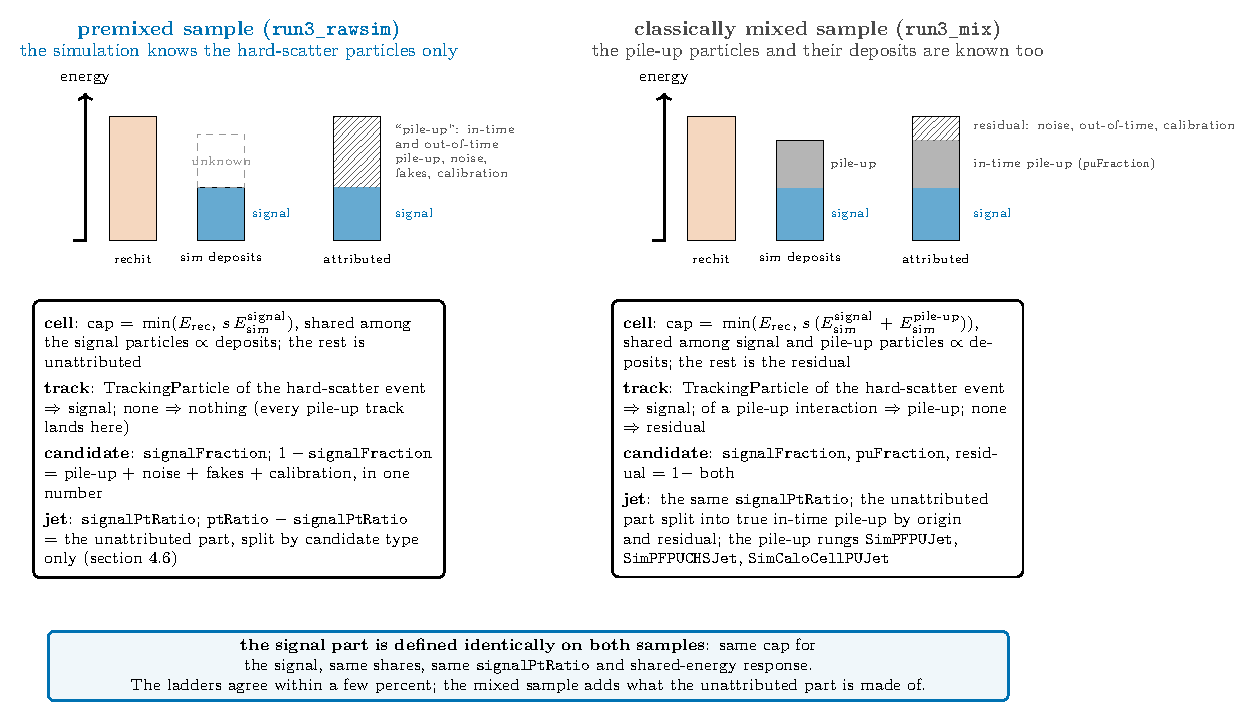
\includegraphics[width=\textwidth]{attribution_samples.pdf}\end{center}

\section*{8. The pile-up truth: classical mixing}
On the premixed samples the pile-up is a pre-digitised library whose particles
are gone, so the remainder of the attribution is "pile-up, noise or fake" as a
whole. Mixing the signal GEN-SIM with minimum-bias GEN-SIM events the classical
way keeps every pile-up particle and deposit, tagged by interaction and
crossing. Every cell is then signal plus known pile-up plus the rest, the
calorimeter scales can be measured cell by cell, the reconstructed candidates
get a pile-up share next to their signal share, and the simulation-level ladder
gets jets with the pile-up in them: the ideal PF of signal plus pile-up, and
the same after a perfect charged-hadron subtraction. The pile-up of a jet is
thereby measured three ways on the same events.
\begin{center}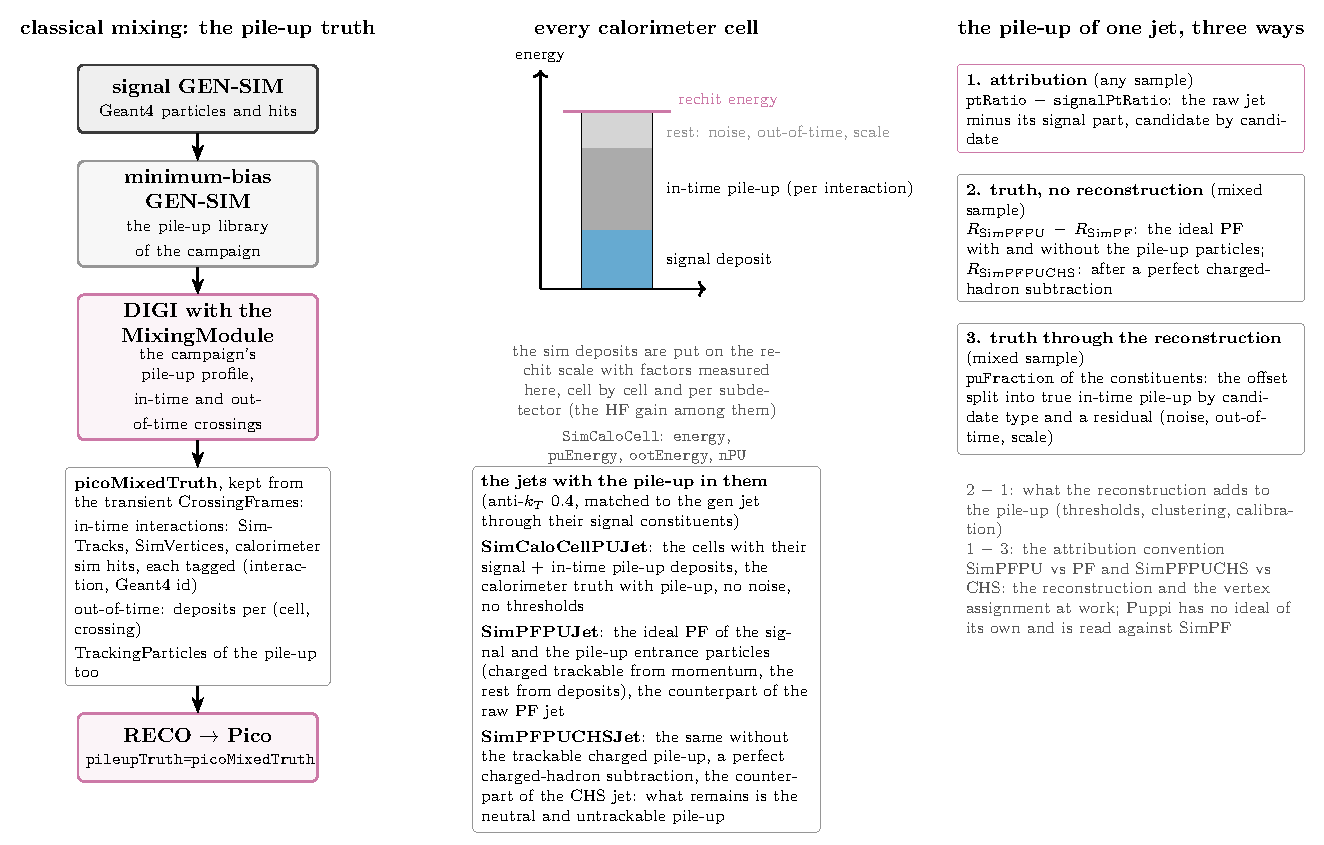
\includegraphics[width=\textwidth]{pileup_truth.pdf}\end{center}

\section*{9. The particle-flow block tables}
For the reconstruction studies the Pico also keeps the full PF block
structure: the elements, the geometric links PF found between them, and the
elements each candidate finally used.
\begin{center}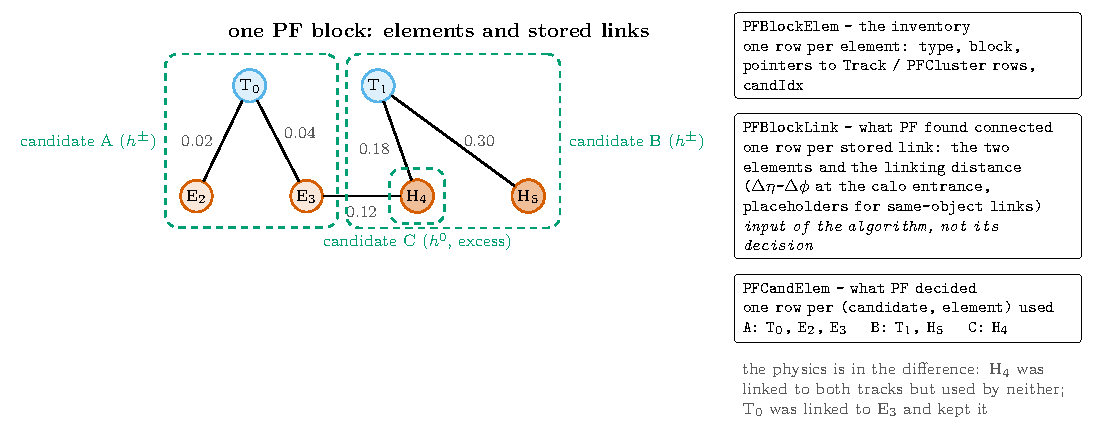
\includegraphics[width=\textwidth]{pf_block.pdf}\end{center}

\section*{Where to read more}
\begin{itemize}
  \item \texttt{Reco2Pico/docs/TrueJES.md}: the physics note
  \item \texttt{Reco2Pico/PicoProducer/README.md}: the table definitions
  \item \texttt{Reco2Pico/analysis/TrueJES/README.md}: the analysis
\end{itemize}
\end{document}
